\section{Cavity Quantum Electrodynamics}

The field of \textit{Cavity Quantum Electrodynamics} explains the interaction between a resonator (in this case a Fabry-Perot cavity), and a piece of matter with which the light inside the resonator interacts with (here: a $^{87}\text{Rb}$ atom). By placing the atom between two highly-reflective mirrors forming the optical cavity, one increases the amount of times a photon that is inside a cavity bounces back and forth between the two mirrors. Increasing the amount of bounces thus effectively increases the cross-section by the number of round-trips the photon takes, allowing for a strong light-matter interaction.\cite{RempeReiserer2015}

The theoretical model which explains this interaction in a fully quantum mechanical picture is called the \textit{Jaynes-Cummings Model} \cite{JaynesCummings1963} and was named after Edwin Jaynes and Fred Cummings who developed it in 1963. For a first look into this model, we'll be considering a three-level-emitter (i.e. our atom), which is interacting with a single cavity optical mode.

The \textit{Jaynes-Cummings} (JC) Model, takes many different quantities into consideration when explaining the interaction and its strength between light and matter.

The photon located in the cavity (which supports only a single optical mode), has a frequency of $\omega_c$. 
Our atom, which is also located in the cavity, supports a transition frequency close to $\omega_c$, from a coupled state $\ket{c}$ and an excited state $\ket{e}$ at a frequency $\omega_a$, which is described in the dipole approximation. 
In order to then complete our three-level-emitter picture, we include an uncoupled state $\ket{u}$ with which the photon does not interact due to this state not being coupled to the cavity light mode.

Lastly, any real atom-cavity system, additionally suffers from losses, those mainly being the spontaneous decay of the atomic excitation at a rate of $2\gamma$, and the damping of the light inside our cavity through the absorption or out-coupling by one of the cavity mirrors at a combined rate of $\kappa$.

The full Hamiltonian which describes interaction between the atom and the cavity thus reads \cite{JC1963}
\begin{equation}
    \mathcal{H_{JC}} = \underbrace{\hbar\omega_{c} \hat{a}^\dag\hat{a}}_{\widehat{=}\text{cavity field}} + \underbrace{\hbar\omega_a \hat{\sigma}_{ce}^\dag\hat{\sigma}_{ce}}_{\widehat{=}\text{atom}} + \underbrace{\hbar g(\hat{a}\hat{\sigma}_{ce}^\dag + \hat{a}^\dag\hat{\sigma}_{ce})}_{\widehat{=}\text{light-atom interaction}}
\label{eq:jc_hamiltonian_simple}
\end{equation}

The three terms in \eqref{eq:jc_hamiltonian_simple} describe the energy of the cavity field, the energy of a bare atom, and the coherent coupling between the two governed by a coupling strength $g$.

The operators $a^\dag$ and $a$ are the creation and annihilation operators of the cavity light modes , whereas $\hat{\sigma}_{ce}=\ket{c}\bra{e}$ and $\hat{\sigma}_{ce}^{\dag}=\ket{e}\bra{c}$ are the atomic raising and lowering operators, respectively.

The form of \eqref{eq:jc_hamiltonian_simple} assumes the so called \textit{Rotating-Wave Approximation} in which fast oscillating terms at optical frequencies can be neglected. 

Solving for the eigenenergies of the system one is left with:

\begin{equation}
    E_\pm (n) = n\hbar\omega_c + \frac{1}{2}\hbar\omega_a \pm \hbar\sqrt{ng^2 + \frac{1}{4}\Delta_{ac}^2}, \quad n\in \mathbb{N}_0
    \label{eq:jc_hamiltonian_eigenenergies}
\end{equation}

The main take-away from \eqref{eq:jc_hamiltonian_eigenenergies} is that on resonance ($\omega_a = \omega_c$), the eigenenergies of the system are split by $2\hbar g\sqrt{n}$, giving rise to the so-called \textit{Vacuum Rabi Splitting}.


\begin{figure}
    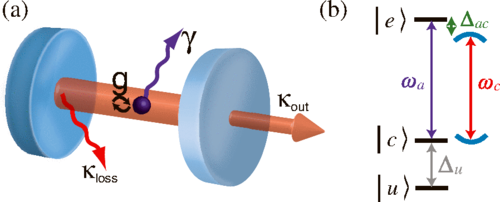
\includegraphics[width=0.7\linewidth]{Figures/theory/jc_setup.png}
    \centering
\end{figure}

\subsection{Birefringent Cavity}

Equation \eqref{eq:jc_hamiltonian_simple} only covers the case for having a single cavity light-mode. The present example however features a birefringent cavity, which is achieved by physically changing the geometric shape of the cavity mirror during production of the fiber ends.\cite{ManuelBThesis2023} This forces a change in the optical path lengths between different polarizations, leading to a frequency splitting $\Delta\nu$ proportional to the ellipticity $\epsilon$ of the mirror surfaces:\cite{UphoffFreqSplit2015}

\begin{equation}
    \Delta\nu = \frac{\nu_{FSR}}{2\pi k}\frac{\epsilon^2}{R_2}.
    \label{eq:freq_split}
\end{equation}

The property $\nu_{FSR}$ in \eqref{eq:freq_split} describes the free spectral range, and $k=\frac{2\pi}{\lambda}$ the photon wavenumber.

This means that we need to consider a system with 2 different light modes for our JC Hamiltonian, which in our case are going to be the $\pi$ and the $V$ modes, whereas we're going to be coupled to the $\pi$ mode, and the $V$ mode will be detuned by $\sim\text{500 MHz}$. This extra consideration can be included in the Hamiltonian as such:

\begin{equation}
    H_{JC} = \hbar\omega_{c,\pi}\hat{a_\pi}^\dag\hat{a_\pi} + \hbar(\omega_{c,\pi}+0.5)\hat{a_V}^\dag\hat{a_V} + \hbar\omega_{a} \hat{\sigma}_{ce}^\dag\hat{\sigma}_{ce} + \hbar g(\hat{a}_\pi\hat{\sigma}_{ce}^\dag + \hat{a}_\pi^\dag\hat{\sigma}_{ce} + \hat{a}_V\hat{\sigma}_{ce}^\dag + \hat{a}_V^\dag\hat{\sigma}_{ce})
    \label{eq:jc_hamiltonian_w_birefringence}
\end{equation}

\subsection{External Drive}
